%%%% IACR Transactions TEMPLATE %%%%
% This file shows how to use the iacrtrans class to write a paper.
% Written by Gaetan Leurent gaetan.leurent@inria.fr (2020)
% Public Domain (CC0)


%%%% 1. DOCUMENTCLASS %%%%
\documentclass[journal=tosc,preprint]{iacrtrans}
%%%% NOTES:
% - Change "journal=tosc" to "journal=tches" if needed
% - Change "submission" to "final" for final version
% - Add "spthm" for LNCS-like theorems


%%%% 2. PACKAGES %%%%
\usepackage{lipsum} % Example package -- can be removed
%%%% 3. AUTHOR, INSTITUTE %%%%
\author{Ajay Tarole\inst{1} \and Ashish Kumar Suraj\inst{2} and Rudraksh Kashyap\inst{3}}
\institute{
  11840090, IIT Bhilai, \email{ajayt@iitbhilai.ac.in}
  \and
  1184230, IIT Bhilai, \email{ashishs@iitbhilai.ac.in}
  \and
  11840970, IIT Bhilai, \email{rudrakshk@iitbhilai.ac.in}
  
}
%%%% NOTES:
% - We need a city name for indexation purpose, even if it is redundant
%   (eg: University of Atlantis, Atlantis, Atlantis)
% - \inst{} can be omitted if there is a single institute,
%   or exactly one institute per author


%%%% 4. TITLE %%%%
\title{PRESENT Cipher}
%%%% NOTES:
% - If the title is too long, or includes special macro, please
%   provide a "running title" as optional argument: \title[Short]{Long}
% - You can provide an optional subtitle with \subtitle.

\begin{document}

\maketitle


%%%% 5. KEYWORDS %%%%
\keywords{PRESENT \and Differential cryptanalysis \and Linear Cryptanalysis}


%%%% 6. ABSTRACT %%%%
\begin{abstract}
	The design of the PRESENT cypher is examined in this work. On the round reduced form of the Cipher, we also examine Differential cryptanalysis, Linear cryptanalysis, and Integral cryptanalysis.  
\end{abstract}


%%%% 7. PAPER CONTENT %%%%
\section{Introduction}
\section{Introduction}
The most prominent algorithms in cryptanalysis are Advanced Encryption Standard (AES) and Data Encryption Standard (DES), as we all know. Both the algorithms have proven resistance against differential and linear cryptoanalysis. The current cypher is a simple cypher.
The current encryption was created with the intention of maximising hardware performance on low-power devices. Linear and Differential cryptanalysis are sensitive to round reduced variants, just as they are to AES. The current cypher is mostly utilised in applications that need little processing resources, such as RFID cards. ISO/IEC 29192-2:2019 is now the standard for the current cypher. 
\section{List of contributions}
\begin{enumerate}
	\item Rudraksh Kashyap: Rudraksh dissected the Present block cipher's design decisions. He also looked at the permutation layer and the S-box or Substitution layer's features. He also implemented the cipher in C. 
	\item Ajay Tarole : Ajay analyed differential cryptanalysis and implemented 3-round reduced  attack using the idea of differential and filtering attack in C.
	\item Ashish Kumar Suraj : Ashish analysed the Linear properties and Integral propetries of the Present Cipher. He also used linear characteristics to examine the resistance of the Present Cipher to linear attacks.  
\end{enumerate}
\section{The Present Cipher}
The PRESENT cipher is a block cipher with block length of 64 bits. The PRESENT cipher supports 80-bit key and 128-bit key. We analyse only 80-bit key version of Present block cipher in our paper. It has a public substitution-box(S-box), bit permutation(P-layer), and key schedule algorithm. The cipher is an Ultra-Lightweight block cipher.\\\\
\subsection{Substitution-Permutation Network}
\begin{figure}[H]
	\centering
	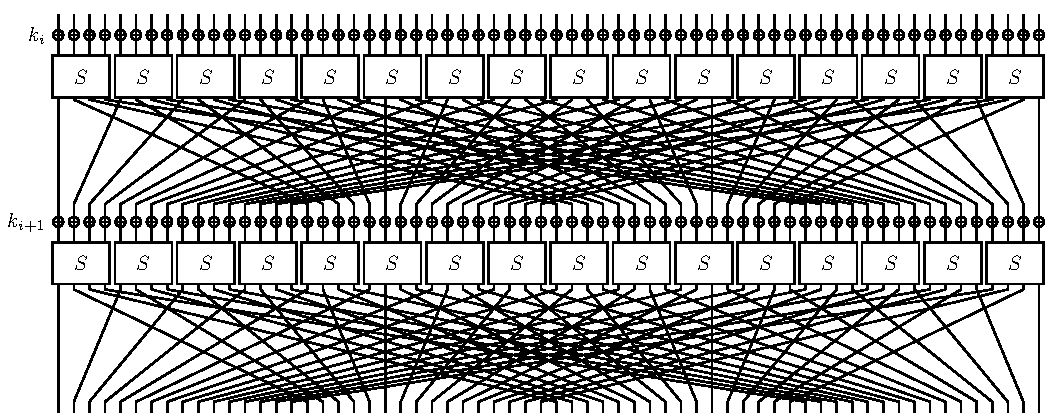
\includegraphics[width=\linewidth]{PRESENT_diagram.pdf}
	\caption{Substitution Permutation Network}
\end{figure}
\subsection{Cipher Design}
The PRESENT-80 bit is part of Substitution and Permutation Network. Figure.2 shows pseudo-code for implementing the encryption of the cipher. The PRESENT cipher has 31 rounds.  Each round consists of a round key, 4-bit substitution layer and linear bit-wise
permutation layer. 
\begin{figure}[h!]
	\centering
	\includegraphics[width=0.34\linewidth, height=0.15\textheight]{"Screenshot from 2021-11-06 08-28-01"}
	\caption{Pseudo Code for PRESENT cipher encryptiom}
	\label{fig:screenshot-from-2021-11-06-08-28-01}
\end{figure}\\

\subsection{Add Round Key}
If the current 64-bit state  is $S = s_{63},s_{62}\dots s_0$ and the 80-bit round key is represented by $K_i = k_{63},k_{62} \dots k_0$ for $1\leq i \leq 32$   then addRoundKey fucntion performs the following operation\\
\hspace*{30mm}$
	S \xrightarrow{} S \oplus K_i \\
\hspace*{20mm}	\implies s_t \xrightarrow[]{} s_t \oplus k_t 
$\\
for $0\leq t\leq 63$.
\subsection{S-Box Layer}
\begin{table}[h!]
\caption{Present sBox}
\centering
\begin{tabular}{ |c||c|c|c|c|c|c|c|c|c|c|c|c|c|c|c|c| }
		\hline
		$x$ & 0 & 1 & 2 & 3&4& 5& 6&7&8&9&A&B&C&D&E&F  \\ \hline
		$SBox[x]$& C & 5 & 6& B &9 &0 &A &D& 3& E &F& 8& 4 &7& 1& 2 \\ \hline
\end{tabular}
\end{table}
The Present S-box has 4-bit to 4-bit mapping in a finite field $F_2^4$. We can see the Present cipher Sbox in Table 1.
\\\\
The Present SBox satisfies the following conditions, due to the avalanche-effect.\\
\begin{enumerate}
	\item For any fixed non-zero input and non-zero ouput difference, $\Delta_I \in \mathbb{F}_2^4$ and $\Delta_O \in \mathbb{F}_2^4$ repectively, we require
	\begin{equation*}
	\#\{ x \in \mathbb{F}_2^4~~ \vert~~ SBox(\Delta_I +x) + SBox(x) = \Delta_O \}| \leq 4
	\end{equation*}
	
	\item For any fixed non-zero input and non-zero ouput difference, $\Delta_I \in \mathbb{F}_2^4$ and $\Delta_O \in \mathbb{F}_2^4$ such that the hamming weight $wt(\Delta_O) = wt(\Delta_I) = 1$ then we have
	\begin{equation*}
	\{ x \in \mathbb{F}_2^4~~ \vert~~  SBox(\Delta_I +x) + SBox(x) = \Delta_O  \} = \Phi
	\end{equation*}
\end{enumerate}
\subsection{P-Layer}
The permutation layer of the cipher  is a bit wise permutation. Here $i^{th}$ bit map with $PLayer(i)^{th}$ bit. The Table 2 show the mapping between bit.
\begin{table}[h!]
	\caption{pLayer}
	\centering
	\begin{tabular}{ |c||c|c|c|c|c|c|c|c|c|c|c|c|c|c|c|c| }
		\hline
		i& 0 &1 &2 &3& 4& 5& 6 &7 &8 &9 &10 &11 &12 &13 &14 &15 \\
		PLayer(i) &0& 16& 32& 48& 1& 17& 33&49& 2 &18& 34& 50& 3 &19 &35 &51 \\\hline\hline
		i &16& 17& 18& 19& 20& 21 &22& 23 &24 &25 &26 &27 &28 &29 &30 &31 \\
		PLayer(i)& 4 &20 &36& 52& 5& 21 &37& 53& 6 &22& 38& 54& 7 &23 &39 &55 \\\hline\hline
		i &32& 33& 34& 35& 36& 37 &38& 39 &40 &41 &42 &43 &44 &45 &46 &47 \\
		PLayer(i) &8 &24& 40& 56 &9& 25 &41 &57 &10 &26 &42 &58 &11 &27 &43 &59 \\\hline\hline
		i &48& 49& 50 &51 &52 &53& 54& 55 &56 &57 &58 &59 &60 &61 &62 &63 \\
		PLayer(i) &12& 28& 44&60& 13 &29& 45& 61 &14 &30 &46 &62 &15 &31 &47 &63 \\\hline
	\end{tabular}
	
\end{table}
\subsection{Key Schedule}
The present can take keys of either 80 or 128 bits. However
we focus on the version with 80-bit keys in this section.
 To begin, the first 80-bit key is placed in a key register $K$ and is denoted by $K = k_{79}k_{78}$...$k_0$. We first take left most 64 bit of of Key register to make $K_i$ that is $i^{th}$ round key as given below:
\begin{equation*}
K_i = \mathrm{k_{63}}\mathrm{k_{62}}..\mathrm{k_{0s}} = k_{79}k_{78}..k_{16}
\end{equation*}
To update the key register $K$, we have to follow the following rules:
\begin{enumerate}
	\item  Each bit of $K$ is rotated to the left by 61 bits. 
	\begin{equation*}
	[k_{79}k_{78}..k_{0}] = [k_{18}k_{17}..k_{20}k_{19}]
	\end{equation*}
	\item 4-leftmost bits of the $K$ we pass in The Present cipher's S-box.
	\begin{equation*}
	[k_{79}k_{78}k_{77}k_{76}] = SBox[k_{79}k_{78}k_{77}k_{76}]
	\end{equation*}
	\item The least significant bits of the round counter value $i$ are exclusive-ored with the 5-bits of key register  $k$, $k_{19}k_{18}k_{17}k_{16}k_{15}$. 
	\begin{equation*}
	[k_{19}k_{18}k_{17}k_{16}k_{15}] = [k_{19}k_{18}k_{17}k_{16}k_{15}] \oplus round-counter
	\end{equation*}
\end{enumerate}
\section{Security Analysis/Attacks}
We presented the results of linear, differential and Integral cryptanalysis of round reduced version of PRESENT cipher, in this section.
\subsection{Differential cryptanalysis}
We'll use $X = x_{15},x_{14},...,x_{1},x_{0}$ to signify the XOR difference of the 16 bits in each step in this section, with $x_15$ being the most important nibble. $K_i$ is the subkey for the $i^{th}$ th round.\\\\ 
Table 3 shows the S-box Difference Distribution Table (DDT).
\begin{table}[h!]
	\caption{DDT of the S-box}
	\centering
	
	\begin{tabular}{ |c||c|c|c|c|c|c|c|c|c|c|c|c|c|c|c|c| }
		\hline
		& 0 & 1 & 2 & 3&4& 5& 6&7&8&9&a&b&c&d&e&f  \\ \hline \hline
		0& 16 & 0 & 0 & 0 &0 &0 &0 &0& 0& 0 &0& 0& 0 &0& 0& 0 \\ 
		1& 0 & 0 & 0 & 4 & 0 & 0 & 0 & 4 & 0 & 4 &0& 0& 0 &4& 0& 0 \\
		2& 0 & 0 & 0 & 2 & 0 & 4 & 2 & 0 & 0 & 0 &2& 0& 2 &2& 2& 0 \\
		3& 0 & 2 & 0 & 2 & 2 & 0 & 4 & 2 & 0 & 0 &2& 2& 0 &0& 0& 0 \\
		4& 0 & 0 & 0 & 0 & 0 & 4 & 2 & 2 & 0 & 2 &2& 0& 2 &0& 2& 0 \\
		5& 0 & 2 & 0 & 0 & 2 & 0 & 0 & 0 & 0 & 2 &2& 2& 4 &2& 0& 0 \\
		6& 0 & 0 & 2 & 0 & 0 & 0 & 2 & 0 & 2 & 0 &0& 4& 2 &0& 0& 4 \\
		7& 0 & 4 & 2 & 0 & 0 & 0 & 2 & 0 & 2 & 0 & 0 & 0 & 2 & 0 & 0 & 4\\
		
		8& 0 & 0 & 0 & 2 & 0 & 0 & 0 & 2 & 0 & 2 & 0 & 4 & 0 & 2 & 0 & 4\\
		9& 0 & 0 & 2 & 0 & 4 & 0 & 2 & 0 & 2 & 0 & 0 & 0 & 2 & 0 & 4 & 0\\
		a& 0 & 0 & 2 & 2 & 0 & 4 & 0 & 0 & 2 & 0 & 2 & 0 & 0 & 2 & 2 & 0\\
		b& 0 & 2 & 0 & 0 & 2 & 0 & 0 & 0 & 4 & 2 & 2 & 2 & 0 & 2 & 0 & 0\\
		c& 0 & 0 & 2 & 0 & 0 & 4 & 0 & 2 & 2 & 2 & 2 & 0 & 0 & 0 & 2 & 0\\
		d& 0 & 2 & 4 & 2 & 2 & 0 & 0 & 2 & 0 & 0 & 2 & 2 & 0 & 0 & 0 & 0\\
		e& 0 & 0 & 2 & 2 & 0 & 0 & 2 & 2 & 2 & 2 & 0 & 0 & 2 & 2 & 0 & 0\\
		f& 0 & 4 & 0 & 0 & 4 & 0 & 0 & 0 & 0 & 0 & 0 & 0 & 0 & 0 & 4 & 4\\ \hline
	\end{tabular}
\end{table}\\
From the properties of the S-box and permutation layer, we will now make some important observations. We divide the 16 S-boxes into 4 groups.\\\\
We can observe the following properties from S-box : 
\begin{enumerate}
	\item The S-Box's input come from four different S-boxes in the same group.  
	\item A group of four S-boxes receives input from 16 separate S-boxes. 
	\item An S-output box's is divided into four different S-boxes for different groups. 
	\item The output of different S-boxes goes to distinct S-boxes. 
\end{enumerate}
\begin{figure}[h!]
	\centering
	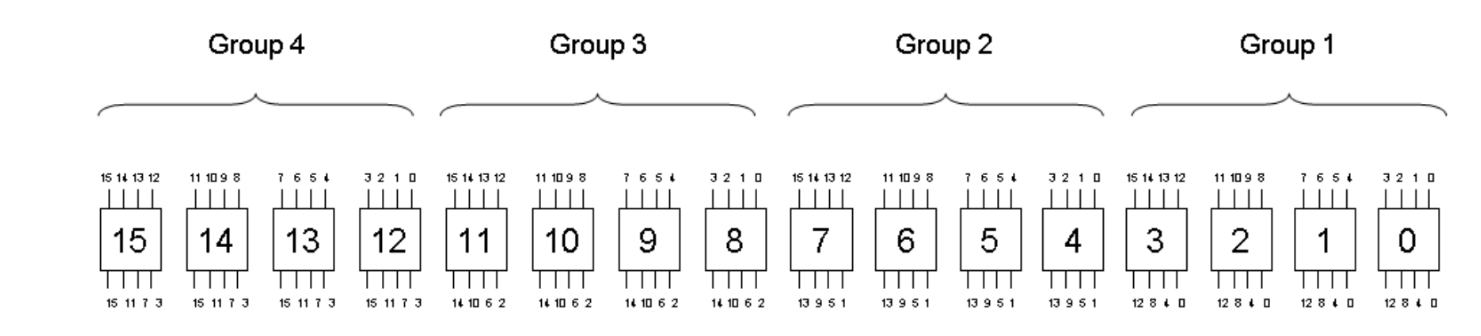
\includegraphics[width=1.0\linewidth, height=0.19\textheight]{groups}
	\caption{Groups of Sboxes}
	\label{fig:groups}
\end{figure}
We may therefore conclude from the previous observations and the Difference Distribution table that a one-bit input difference will result in at least two-bit output difference.
The differential uniformity is maximum at 4 and the differential probability is maximum at $2^{-2}$. 
\subsection{Differential Characteristics}
\begin{figure}[h!]
	\centering
	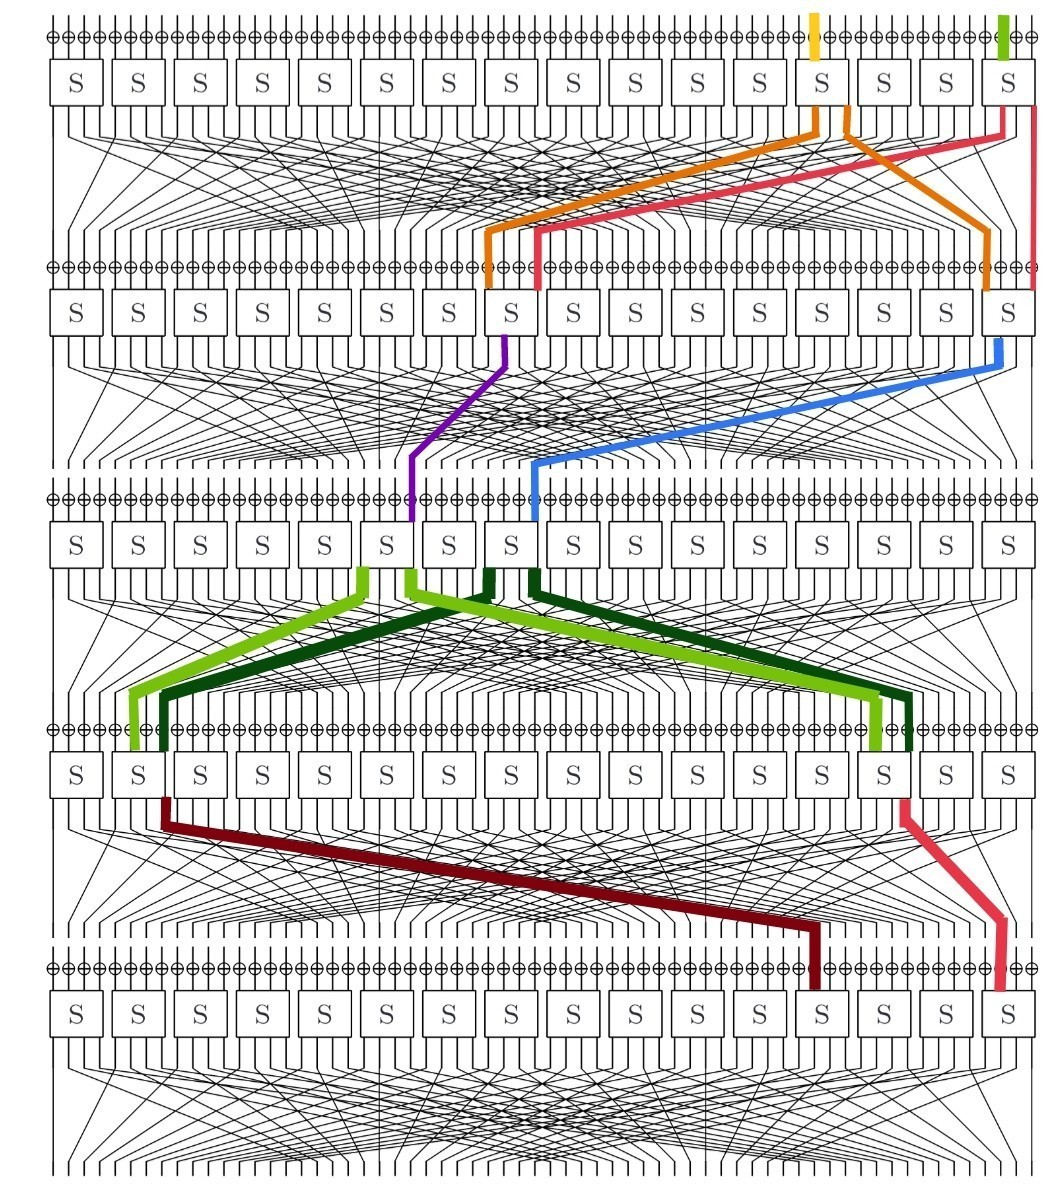
\includegraphics[width=0.6\linewidth, height=0.5\textheight]{IMG_20211114_110332}
	\caption{Probability we have to pay in four round characteristics is $2^{-18}$}
	\label{fig:img20211114110332}
\end{figure}
\newpage
\begin{table}[h!]
	\caption{Round wise probability we have to pay}
	\centering
	\begin{tabular}{ |c||c|c|c| }
		\hline
		Rounds & & Diff. & Prob. \\ \hline \hline
		I& & $x_3 = 4$, $x_0 = 4$ &  \\ 
		$R_1$& SBox & $x_3 = 5$, $x_{0} = 5$ & $2^{-4}$ \\
		$R_1$& PLayer & $x_8 = 9$, $x_{0} = 9$ & 1 \\
		$R_2$& SBox & $x_8 = 4$, $x_{0} = 4$ & $2^{-4}$ \\
		$R_2$& PLayer & $x_{10} = 1$, $x_{8} = 1$ & 1 \\
		$R_3$& SBox & $x_{10} = 9$, $x_{8} = 9$ & $2^{-4}$ \\
		$R_3$& PLayer & $x_{14} = 5$, $x_{2} = 5$ & 1 \\
		$R_4$& SBox & $x_{14} = 1$, $x_{2} = 1$  & $2^{-6}$ \\
		$R_4$& PLayer & $x_4 = 4$, $x_0 = 4$ & 1 \\ \hline
	\end{tabular}\\
\end{table}
Here we are paying $2^{-18}$ probality and we will reach to our initial input $x_3 = 4$ and $x_0 = 4$ after 4 rounds. Now using the above diffirencial charateristics we can reach next four round(5-8) by paying another $2^{-18}$ probability. So overall we found 8 round iterative diffirencial charateristics with probability $2^{-36}$. For 12 rounds we have to pay $2^{-54}$ and for 14 round we have to pay $2^{-62}$ probability.
\subsection{Attack}
In this section, we implement or analize attack on three-round reduced PRESENT cipher.
For this attack, we use $2^{18}$ chosen plain text pairs. Only 2 active S-boxes $(S_0 $ and $S_3)$ in the first round. Only two bit input difference in plaintext pairs at position 0th bit and 14th bit. Other S-boxes in the first round is inctive. \\\\
\textbf{Round Reduced Attack:}\\
\begin{figure}[h!]
	\centering
	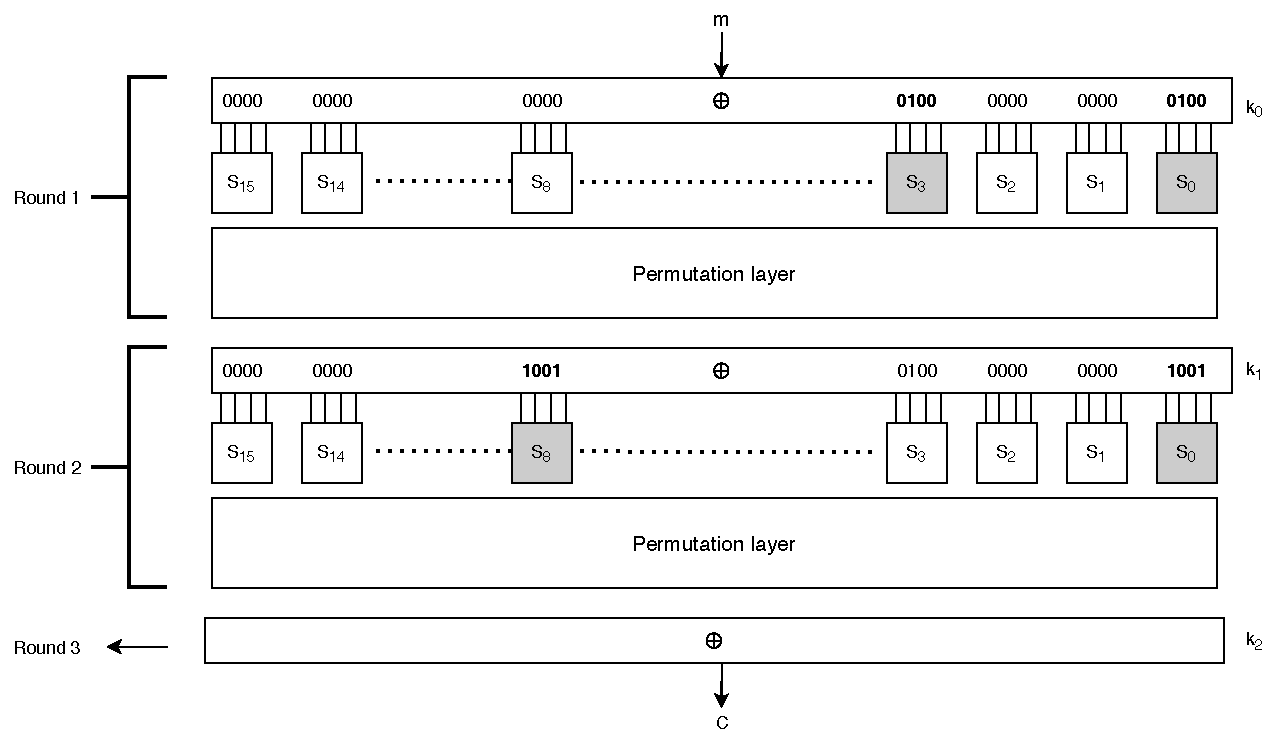
\includegraphics[width=0.9\linewidth, height=0.3\textheight]{DC1}
	\caption{Attack on 3-Round Reduced PRESENT Cipher}
	\label{fig:dc1}
\end{figure}\\
\textbf{Characteristic:}\\\\
\begin{table}[h!]
	\caption{Characteristics}
	\centering
	\begin{tabular}{ |c||c|c|c| }
		\hline
		Rounds & & Diff. & Prob. \\ \hline \hline
		I& & $x_0 = 4$, $x_4 = 4$ &  \\ 
		$R_1$& $k_0$ & $x_0 = 4$, $x_4 = 4$ & 1 \\
		$R_1$& SBox & $x_0 = 5$, $x_{3} = 5$ & $2^{-4}$ \\
		$R_1$& PLayer & $x_0 = 9$, $x_{8} = 9$ & 1 \\
		$R_2$& $k_1$ & $x_0 = 9$, $x_{8} = 9$ & 1 \\ \hline
	\end{tabular}\\
\end{table}
	($x_0 = 4$, $x_3 = 4$) $\xrightarrow[]{\text{R}}$ ($x_0 = 9$, $x_8 = 9$)\\\\
\textbf{Idea of filtering:}\\
1. Decrease Wrong pair $\rightarrow$ Idea of filtering\\
2. Observe from the DDT that transitions from
	9 $\rightarrow$ {2, 4, 6, 8, c, e}\\
3. Thus, after the effect of permutation layer of the second round, $c_1 \oplus c_2$ must belong to the set given below : \\ 
$\{\{x_4=1,x_6=1\},\{x_6=1,x_8=1\},\{x_4=1,x_6=1,x_8=1\},\{x_6=1,x_{12}=1\},\{x_6=1,x_8=1,x_{12}=1\},...\}$ We have written code for this.\\\\
Note: Thus, message pair leading to the cipher text difference other than the above set, can be discarded. \\\\
So, after filtering only $2^{14}$ plaintext pairs are left in our case.\\\\
\textbf{Key Guess:}\\
\begin{figure}[h!]
	\centering
	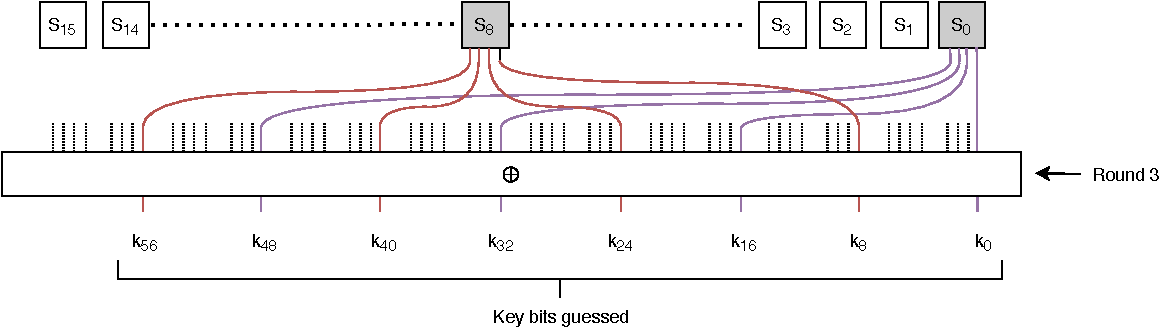
\includegraphics[width=0.9\linewidth, height=0.2\textheight]{DC2}
	\caption{Guess 8 bits of the key $k_2$}
	\label{fig:dc2}
\end{figure}\\
We are able to find 8 bits of key $k_2$. In our case only  8 bit right  subkey holds for all $2^{14}$ filtered pairs.
\subsection{Analysing the attack}
\textbf{Complexity Analysis:}\\\\
\textbf{Data:} $2^{18}$ plaintext pairs or $2^{19}$ plaintexts\\\\
\textbf{Memory:} $2^{14}$ array used to store filtered pairs\\\\
\textbf{Time:} \\\\ 
Filtering: \\
2 round encryption of $2^{18}$ plaintext pairs and compare every pairs with set of 36 possible ciphertext that we are using for filtering. \\\\
$36 \times ({2 \times 2 \times 2^{18}}) = 2^{5.17} \times 2^{20} = 2^{25.17}$\\\\
Attack:\\
2 round encryption of $2^{14}$ filtered plaintext pairs  then $2^{6}$ key gueses and $2^{14}$  ciphertext pairs decrypt for 1 round.\\\\
$2 \times (2 \times 2^{14}) + 2^6 \times (2 \times 2^{14}) = 2^{16} + 2^{21} \approx 2^{22} $\\\\
\textbf{(Data, Time, Memory)} = $(2^{19},2^{25.17},2^{14})$\\\\\\
\subsection{Linear cryptanalysis}
In this part, we will analyse at Present cipher's linear approximation. First, we'll go over the PRESENT Linear Approximation Table:\\
\begin{table}[h!]
	\centering
	\caption{LAT of the S-box}
	\begin{tabular}{ |c||c|c|c|c|c|c|c|c|c|c|c|c|c|c|c|c| }
		\hline
		& 0 & 1 & 2 & 3&4& 5& 6&7&8&9&a&b&c&d&e&f  \\ \hline \hline
		0& 8 & 0 & 0 & 0 & 0 & 0 & 0 & 0 & 0 & 0 & 0 & 0 & 0 & 0 & 0 & 0 \\ 
		1& 0 & 0 & 0 & 0 & 0 & -4 & 0 & -4 & 0 & 0 & 0 & 0 & 0 & -4 & 0 & 4 \\
		2& 0 & 0 & 2 & 2 & -2 & -2 & 0 & 0 & 2 & -2 & 0 & 4 & 0 & 4 & -2 & 2 \\
		3& 0 & 0 & 2 & 2 & 2 & -2 & -4 & 0 & -2 & 2 & -4 & 0 & 0 & 0 & -2 & -2 \\
		4& 0 & 0 & -2 & 2 & -2 & -2 & 0 & 4 & -2 & -2 & 0 & -4 & 0 & 0 & -2 & 2 \\
		5& 0 & 0 & -2 & 2 & -2 & 2 & 0 & 0 & 2 & 2 & -4 & 0 & 4 & 0 & 2 & 2\\
		6& 0 & 0 & 0 & -4 & 0 & 0 & -4 & 0 & 0 & -4 & 0 & 0 & 4 & 0 & 0 & 0\\
		7& 0 & 0 & 0 & 4 & 4 & 0 & 0 & 0 & 0 & -4 & 0 & 0 & 0 & 0 & 4 & 0\\
		8& 0 & 0 & 2 & -2 & 0 & 0 & -2 & 2 & -2 & 2 & 0 & 0 & -2 & 2 & 4 & 4\\
		9& 0 & 4 & -2 & -2 & 0 & 0 & 2 & -2 & -2 & -2 & -4 & 0 & -2 & 2 & 0 & 0\\
		a& 0 & 0 & 4 & 0 & 2 & 2 & 2 & -2 & 0 & 0 & 0 & -4 & 2 & 2 & -2 & 2\\
		b& 0 & -4 & 0 & 0 & -2 & -2 & 2 & -2 & -4 & 0 & 0 & 0 & 2 & 2 & 2 & -2\\
		c& 0 & 0 & 0 & 0 & -2 & -2 & -2 & -2 & 4 & 0 & 0 & -4 & -2 & 2 & 2 & -2\\
		d& 0 & 4 & 4 & 0 & -2 & -2 & 2 & 2 & 0 & 0 & 0 & 0 & 2 & -2 & 2 & -2\\
		e& 0 & 0 & 2 & 2 & -4 & 4 & -2 & -2 & -2 & -2 & 0 & 0 & -2 & -2 & 0 & 0\\
		f& 0 & 4 & -2 & 2 & 0 & 0 & -2 & -2 & -2 & 2 & 4 & 0 & 2 & 2 & 0 & 0\\
		\hline
	\end{tabular}
\end{table}\\
Now The LAT of the PRESENT S-box has a few interesting features. Let's go through them:
\begin{itemize}
	\item Maximum bias of all linear approximations $ \le 2^{-2}$
	\item Maximum linear approximation of a single bit is $\le 2^{-3}$
\end{itemize}
   Using the preceding data, we first attempt to constrain the bias of four rounds of PRESENT. Remember the piling up lemma, which states that the probability of linear approximation for n separate occurrences for n S-boxes is given by:
\begin{equation*}
\frac{1}{2} + 2^{n-1} \prod_{i=1}^{n} \left( p_i  - \frac{1}{2} \right)
\end{equation*}\\
So, the bias can be given by:
\begin{equation*}
2^{n-1}\prod_{i=1}^{n} \epsilon_i
\end{equation*}
Each of the four rounds the number of active S-boxes can vary. So, we have three case to compute number of active S-boxes ( Let the bias $\epsilon_4^{(i)}$ here i active sbox active in 4 round of Present Cipher.) : 
\begin{enumerate}
	\item  Let's say there are four active S-boxes in total, with one active S-box in each round. As shown in figure 7. The maximum bias of each middle round is at most $2^{-3}$ if two active S-boxes are there. And the bias of the first and last round is at most $2^{-2}$. 
	
    \begin{figure}[h!]
	\centering
	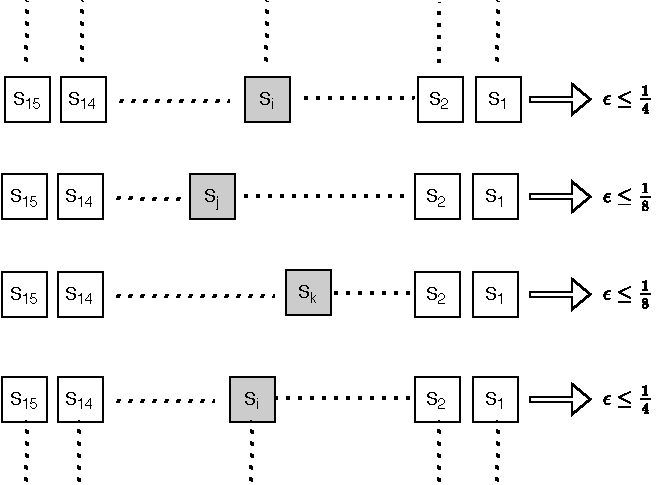
\includegraphics[width=0.7\linewidth, height=0.4\textheight]{LC}
	\caption{Four rounds characteristics}
	\label{fig:lc}
    \end{figure}
As a result, the case's bias is limited: 	\begin{equation*}
	\epsilon_4^{(4)} \leq 2^{4-1} \times (2^{-2})^2 \times (2^{-3})^2
	\end{equation*}
	\begin{equation*}
	\epsilon_4^{(4)} \leq 2^{-7} 
	\end{equation*}
	\item Let's say there are 5 S-boxes involved in each of the four rounds. The active S-box pattern can not then be 1-2-1-1 or 1-1-2-1. Because the two active S-boxes are begun by the same S-box in the previous round, we know they must belong to two different groups based on the prior findings. As a result, they'll turn on at least two S-boxes in the next round. As a result, the bias is constrained by: 2-1-1-1 or 1-1-1-2 as a feasible pattern for this scenario:
	\begin{equation*}
	\epsilon_4^{(5)} \leq 2^{5-1} \times (2^{-2})^4 \times (2^{-3})
	\end{equation*}
	\begin{equation*}
	\epsilon_4^{(5)} \leq 2^{-7} 
	\end{equation*}
	\item Allow for a total of more than 5 active S-boxes. The maximum bias in this scenario is $\frac{1}{4}$ for each round. As a result,: 
	\begin{equation*}
	\epsilon_4^{(i)} \leq 2^{i-1} \times (2^{-2})^i \;\; for \;\; i > 5
	\end{equation*}
	For $i = 6$, the bias is clearly equal to $2^{-7}$, and for $i>6$, the bias is strictly smaller than $2^{-7}$. 
\end{enumerate}
As a result of the aforementioned research, we can say that for 4-rounds of linear approximation of the present cipher the bias is given by $2^{-7}$,
Using above result we can calculate the the linear approximation bias for all 28 rounds of the present cipher.
 \begin{equation*}
\epsilon_{28} \leq 2^{6} \times \epsilon_4^{7} = 2^6 \times (2^{-7})^7 \implies \epsilon_{28} \leq 2^{-43}
\end{equation*}
For a single bit recovery, $N = c|\epsilon|^{-2}$ gives a decent approximation of the number of known plain-texts (N) needed for a successful assault.
The attacker will need to approximate 28 rounds of PRESENT, to attack 31 rounds of PRESENT. So, he need $2^{86}$ plaintexts. This is even more than the $2^{64}$ of accessible space. \\\\
\textbf{Two round characteristics:}
\begin{figure}[h!]
	\centering
	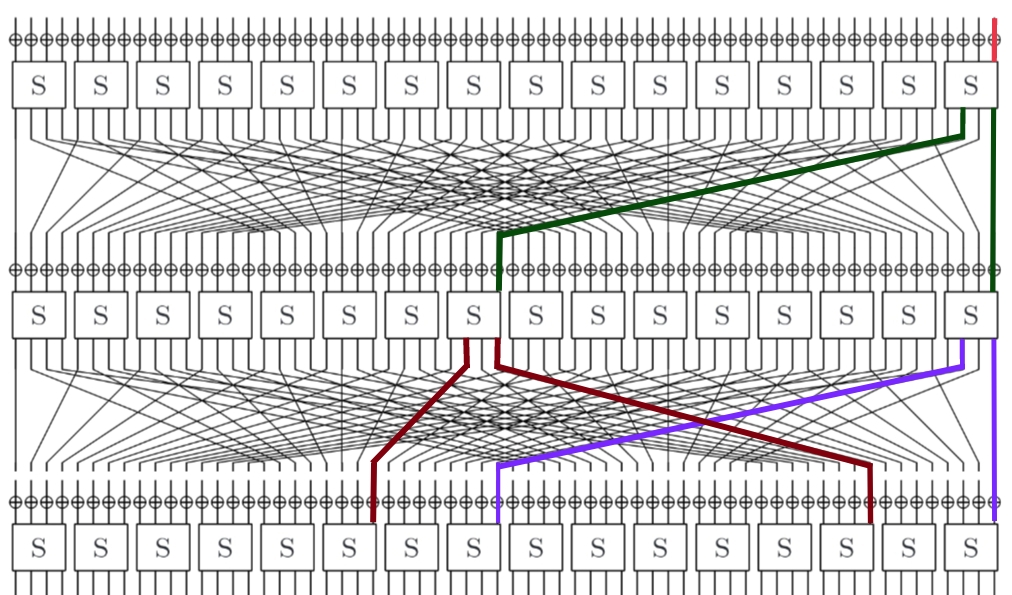
\includegraphics[width=1.0\linewidth, height=0.32\textheight]{LC2}
	\caption{Two round characteristics}
	\label{fig:lc2}
\end{figure}\\
\textbf{Characteristic:}\\\\
	($x_0 = 1$) $\xrightarrow[]{\text{R}}$ ($x_0 = 1$, $x_8 = 1$)$\xrightarrow[]{\text{R}}$ ($x_0 = 1$, $x_2 = 1$,$x_8 = 1$, $x_{10} = 1$)\\\\
	$p_1= \frac{1}{2}-\frac{4}{16}=\frac{1}{4}$\\\\
	$p_2=\frac{1}{2}+2(\frac{4}{16})^2=\frac{1}{2}+\frac{1}{8}=\frac{5}{8}$\\\\\\
	Probability of 2-round Characteristics:\\\\
	$\frac{1}{4} \times \frac{5}{8}+\frac{3}{4} \times \frac{3}{8}=\frac{7}{16}=\frac{1}{2}-\frac{1}{16}$\\
\begin{table}[h!]
	\caption{Characteristics}
	\centering
	\begin{tabular}{ |c||c|c|c| }
		\hline
		Rounds & & Diff. & Prob. \\ \hline \hline
		I& & $x_0 = 1$ &  \\ 
		$R_1$& $k_0$ & $x_0 = 1$ & 1 \\
		$R_1$& S & $x_0 = 5$ & $2^{-2}$ \\
		$R_1$& P & $x_0 = 1$, $x_{8} = 1$ & 1 \\
		$R_2$& $k_1$ & $x_0 = 1$, $x_{8} = 1$ & 1 \\
		$R_2$& S & $x_0 = 5$,$x_8 = 5$ & $2^{-4}$ \\
		$R_2$& P & $x_0 = 1$, $x_2 = 1$, $x_8 = 1$, $x_{10} = 1$ & 1 \\
		$R_3$& $k_1$ & $x_0 = 1$, $x_2 = 1$, $x_8 = 1$, $x_{10} = 1$ & 1 \\
		 \hline
	\end{tabular}\\
\end{table}
\section{Integral cryptanalysis}
In this section, we will analyze 5-round integral distinguishers for PRESENT.\\\\
\textbf{5 round distinguishers:}\\\\
In distinguisher, if we fix the left most 60 bits as random constant and theb vary 4 right most bits, then after five round encryption, the four right most bits of the state are balanced.\\\\
Input: (ccccccccccccccccccccccccccccccccccccccccccccccccccccccccccccaaaa)\\
Ouput:(????????????????????????????????????????????????????????bbbb)\\\\
c: constant bit, a: active bit, b: balanced bit, ?: unknown bit\\\\
We have run this distinguisher for $2^{12}$ different messages. The experiment result return the four right most bits as balanced bits. We right the c code to verify this distinguisher.
\section{Conclusions}
 We have discussed the working mechanism of the PRESENT Cipher. Then we implemented  the Present cipher of 80 bit key version in C language. Then we analyse the S-box's properties. Then we implemented three-round reduced differential attack on the Present cipher in c. We also verified and implemented 5 Rounds integral property of PRESENT in c. We have also analysed DDT and LAT.
\section{Brownie Point Nomination}
\begin{enumerate}
	\item We implemented three-rounds reduced differential attack on the PRESENT cipher. 
	\item We have verified 5 Rounds integral property of PRESENT.
\end{enumerate}
%%%% 8. BILBIOGRAPHY %%%%
%\bibliographystyle{alpha}
%\bibliography{abbrev3,crypto,biblio}
%%%% NOTES
% - Download abbrev3.bib and crypto.bib from https://cryptobib.di.ens.fr/
% - Use bilbio.bib for additional references not in the cryptobib database.
%   If possible, take them from DBLP.
\begin{thebibliography}{}
	\bibitem{} A. BogdanovL. R. KnudsenG. LeanderC. PaarA. PoschmannM. J. B. RobshawY. SeurinC. Vikkelsoe. "PRESENT: An Ultra-Lightweight Block Cipher" (2007). 
	URL:  \href{https://link.springer.com/chapter/10.1007/978-3-540-74735-2_31} {https://link.springer.com/chapter/10.1007/978-3-540-74735-2\_31}
	\bibitem{} Meiqin Wang. "Differential Cryptanalysis of Reduced-Round PRESENT" (2008). URL: \href{https://link.springer.com/chapter/10.1007/978-3-540-68164-9_4}{https://link.springer.com/chapter/10.1007/978-3-540-68164-9\_4}
	\bibitem{} Onur ÖzenKerem VarıcıCihangir TezcanÇelebi Kocair. "Lightweight Block Ciphers
	Revisited: Cryptanalysis of Reduced Round PRESENT and HIGHT" (2009). URL: \href{https://link.springer.com/chapter/10.1007/978-3-642-02620-1_7}{https://link.springer.com/chapter/10.1007/978-3-642-02620-1\_7}
	\bibitem{} Kenji Ohkuma. "Weak Keys of Reduced-Round PRESENT for Linear Cryptanalysis"
	(2009).URL: \href{https://link.springer.com/chapter/10.1007/978-3-642-05445-7_16}{https://link.springer.com/chapter/10.1007/978-3-642-05445-7\_16}
	\bibitem{} Joo Yeon Cho. "Linear Cryptanalysis of Reduced-Round PRESENT" (2010). URL: \href{https://link.springer.com/chapter/10.1007/978-3-642-11925-5_21}{https://link.springer.com/chapter/10.1007/978-3-642-11925-5\_21}
	\bibitem{} Julia Borghoff Lars R. Knudsen Gregor Leander Soren S. Thomsen. "Cryptanalysis
	of PRESENT-like ciphers with secret S-boxes" (2010). URL: \href{https://core.ac.uk/download/pdf/189797554.pdf}{https://core.ac.uk/download/pdf/189797554.pdf}
	\bibitem{} Jan Pospíšil; Martin Novotný. "Lightweight cipher resistivity against brute-force
	attack: Analysis of PRESENT" (2012). URL: \href{https://ieeexplore.ieee.org/abstract/document/6219055}{https://ieeexplore.ieee.org/abstract/document/6219055}
	\bibitem{} Chen-Hui Jin Guo-Qiang Liu. "Differential cryptanalysis of PRESENT-like cipher"
	(2014). URL: \href{https://link.springer.com/article/10.1007/s10623-014-9965-1}{https://link.springer.com/article/10.1007/s10623-014-9965-1}
	\bibitem{} Davide Bellizia; Giuseppe Scotti; Alessandro Trifiletti. "Implementation of the
	PRESENT-80 block cipher and analysis of its vulnerability to Side Channel Attacks
	Exploiting Static Power" (2016). URL: \href{https://ieeexplore.ieee.org/abstract/document/7529734}{https://ieeexplore.ieee.org/abstract/document/7529734}
	\bibitem{} Thomas De Cnudde; Svetla Nikova. "Securing the PRESENT Block Cipher Against
	Combined Side-Channel Analysis and Fault Attacks" (2017). URL: \href{https://ieeexplore.ieee.org/abstract/document/7956221}{https://ieeexplore.ieee.org/abstract/document/7956221}
\end{thebibliography}

\end{document}
